\newpage
\section{Wasserkraft}


\subsection{Kontinuitätsgleichung des Durchflusses}
\begin{center}
    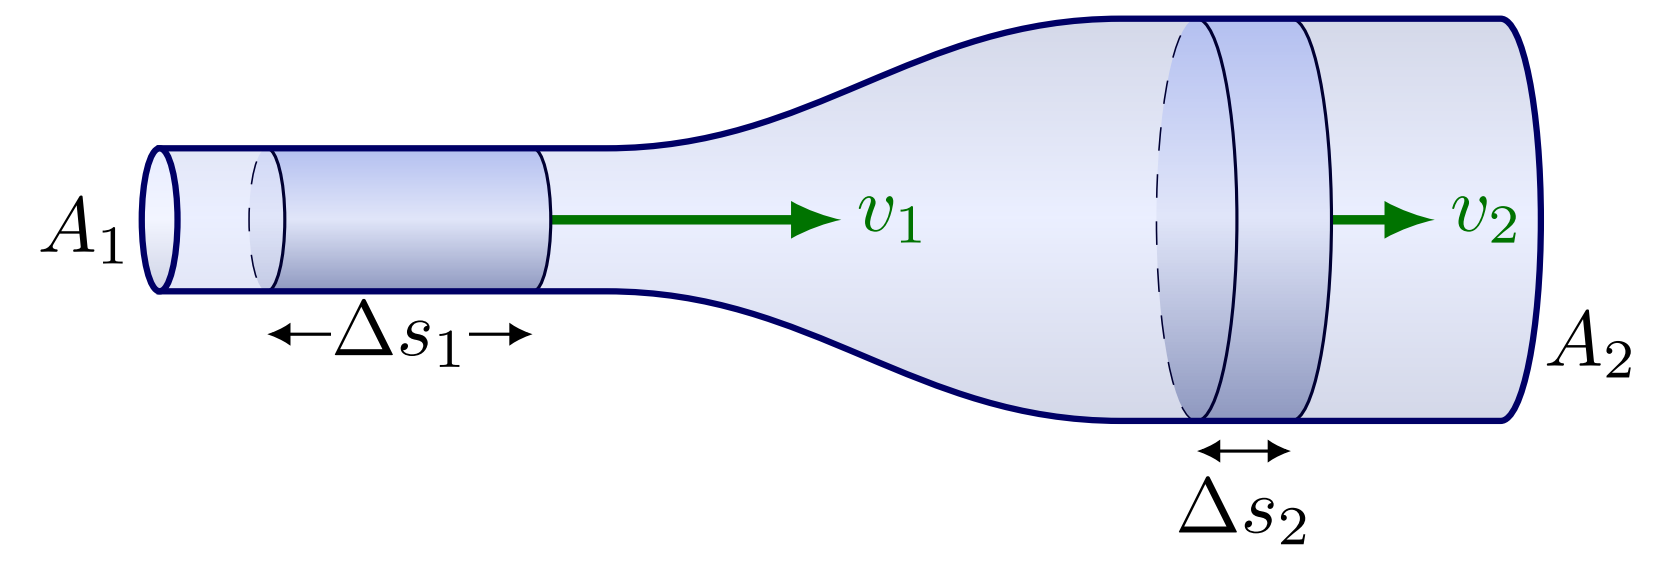
\includegraphics[width=0.9\columnwidth, align=c]{images/Kontinuitaet.png}
\end{center}

Die Kontinuitätsgleichung beschreibt die Erhaltung des Volumenstroms in einer strömenden Flüssigkeit:

\vspace{0.15cm}

$
\boxed{
    Q = A \cdot v 
} 
\quad
\boxed{
    Q_1 = Q_2 
} 
\quad
\boxed{
    A_1 \cdot v_1 = A_2 \cdot v_2
}
\quad
\boxed{
    Q = \dot{V} = \frac{\Delta V}{\Delta t} = \text{const} 
} 
$

\vspace{0.15cm}

\renewcommand{\arraystretch}{1.2} % Erhöht Zeilenhöhe für bessere Lesbarkeit
\begin{tabular}{@{} l p{6cm} l @{}}
    $[Q_x]$        & Durchflussrate                     \dotfill & $\mathrm{\frac{m^3}{s}}$ \\
    $[A_x]$        & Querschnittsfläche                 \dotfill & $\mathrm{m^2}$ \\
    $[v_x]$        & Fliessgeschwindigkeit              \dotfill & $\mathrm{\frac{m}{s}}$ \\
    $[\dot{V}]$    & Volumenstrom (Volumen pro Zeit)    \dotfill & $\mathrm{\frac{m^3}{s}}$ \\
    $[\Delta V]$   & Volumenänderung                    \dotfill & $\mathrm{m^3}$ \\
    $[\Delta t]$   & Zeitänderung                       \dotfill & $\mathrm{s}$ \\
\end{tabular}



\subsection{Bernoulli-Druck-Gleichung für Speicherwasserkraftwerke}

\begin{center}
    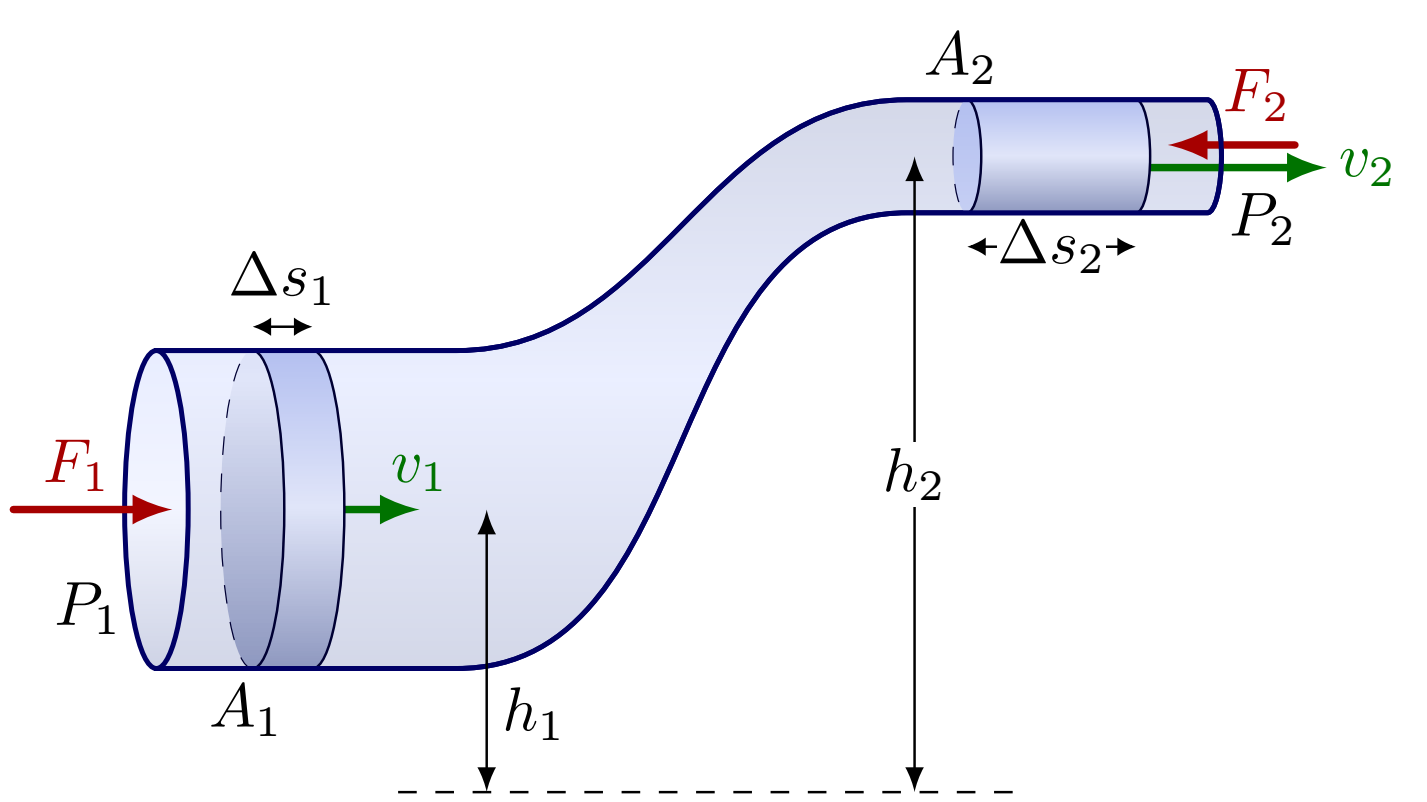
\includegraphics[width=0.9\columnwidth, align=c]{images/Bernoulli.png}
\end{center}

$\boxed{\frac{1}{2} \cdot \rho \cdot v^2 + \rho \cdot g \cdot z + p = \text{constant}}$

\vspace{0.15cm}

$
\boxed{
p_1 + \rho \cdot g \cdot h_1 + \frac{1}{2} \rho \cdot v_1^2 
= 
p_2 + \rho \cdot g \cdot h_2 + \frac{1}{2} \rho \cdot v_2^2
}
$

\vspace{0.15cm}

\renewcommand{\arraystretch}{1.2} % Erhöht Zeilenhöhe für bessere Lesbarkeit
\begin{tabular}{@{} l p {6cm} l @{}}
    $[\frac{1}{2} \rho v^2]$ & Kinetische Energie (je Kubikmeter) \dotfill & $\mathrm{\frac{J}{m^3}}$ \\
    $[\rho g z]$             & Potentielle Energie                 \dotfill & $\mathrm{\frac{J}{m^3}}$ \\
    $[p]$                    & Druckenergie                        \dotfill & $\mathrm{\frac{J}{m^3}}$ \\
\end{tabular}


\vspace{0.15cm}

$
\underbrace{p}_{A} + \underbrace{\rho g z}_{B} + \underbrace{\frac{1}{2}\rho v^2}_{C} = \underbrace{\text{constant}}_{D}
$


\subsection{Bernoulli-Höhen-Gleichung für Speicherwasserkraftwerke}

$\boxed{H = z + \frac{p}{\rho \cdot g} + \frac{v^2}{2 \cdot g} + \sum H_v}$

\vspace{0.15cm}

\renewcommand{\arraystretch}{1.2} % Erhöht Zeilenhöhe für bessere Lesbarkeit
\begin{tabular}{@{} l p {4cm} l @{}}
    $[H]$                           & Bruttogefälle                              \dotfill & $\mathrm{m}$ \\
    $[z]$                           & Höhenlage (potenzielle Energie)            \dotfill & $\mathrm{m}$ \\
    $[p]$                           & Druck                                      \dotfill & $\mathrm{Pa} = \mathrm{\frac{N}{m^2}}$ \\
    $[\rho]$                        & Dichte des Wassers                         \dotfill & $\mathrm{\frac{kg}{m^3}}$ \\
    $[g]$                           & Erdbeschleunigung                          \dotfill & $\mathrm{\frac{m}{s^2}}$ \\
    $[v]$                           & Geschwindigkeit                            \dotfill & $\mathrm{\frac{m}{s}}$ \\
    $\left[\frac{p}{\rho g}\right]$ & Druckhöhe                                  \dotfill & $\mathrm{m}$ \\
    $\left[\frac{v^2}{2g}\right]$   & Geschwindigkeitshöhe                       \dotfill & $\mathrm{m}$ \\
    $[\sum H_v]$                    & Hydraulische Energieverluste               \dotfill & $\mathrm{m}$ \\
\end{tabular}



\subsection{Örtliche Energieverluste}

$\boxed{h_v = \zeta \cdot \frac{v^2}{2g}}$

\vspace{0.15cm}

\renewcommand{\arraystretch}{1.2} % Erhöht Zeilenhöhe für bessere Lesbarkeit
\begin{tabular}{@{} l p {4cm} l @{}}
    $[h_v]$     & Örtliche Energieverlusthöhe   \dotfill & $\mathrm{m}$ \\
    $[\zeta]$   & Verlustbeiwert (dimensionslos) \dotfill & $-$ \\
    $[v]$       & Geschwindigkeit               \dotfill & $\mathrm{\frac{m}{s}}$ \\
    $[g]$       & Erdbeschleunigung             \dotfill & $\mathrm{\frac{m}{s^2}}$ \\
\end{tabular}



\subsection{Reibungsverluste (Formel von Strickler)}

$\boxed{h_{\text{v,r}} = \frac{v^2 \cdot L}{K_{St}^2 \cdot R_h^{4/3}}}$

\vspace{0.15cm}

\renewcommand{\arraystretch}{1.2} % Erhöht Zeilenhöhe für bessere Lesbarkeit
\begin{tabular}{@{} l p {4cm} l @{}}
    $[h_{\text{v,r}}]$  & Reibungsverlusthöhe           \dotfill & $\mathrm{m}$ \\
    $[v]$               & Strömungsgeschwindigkeit      \dotfill & $\mathrm{\frac{m}{s}}$ \\
    $[L]$               & Länge der Strömungsstrecke    \dotfill & $\mathrm{m}$ \\
    $[K_{St}]$          & Rauhigkeitsbeiwert nach Strickler \dotfill & $\mathrm{\frac{m^{1/3}}{s}}$ \\
    $[R_h]$             & Hydraulischer Radius          \dotfill & $\mathrm{m}$ \\
\end{tabular}



\subsubsection{Tabelle Rauhigkeitsbeiwert $K_{St}$ nach Strickler}
\begin{tabular}{|l|l|c|}
    \hline
    \textbf{Material} & \textbf{Zustand} & \textbf{$K_{St}$ [m$^{1/3}$/s]} \\
    \hline
    Stahl & neu & 75 \\
    \hline
    Stahl & schlechter Zustand, verrostet, verkrustet & 60 \\
    \hline
    Beton & glatt & 85 \\
    \hline
    Beton & rauh & 60 \\
    \hline
    PE, PVC &  & 100 \\
    \hline
\end{tabular}


\subsubsection{Hydraulischer Radius}

\begin{minipage}[c]{0.48\columnwidth}
    \myul{\textbf{Rechteckqueerschnitt}}\\
    \begin{center}
        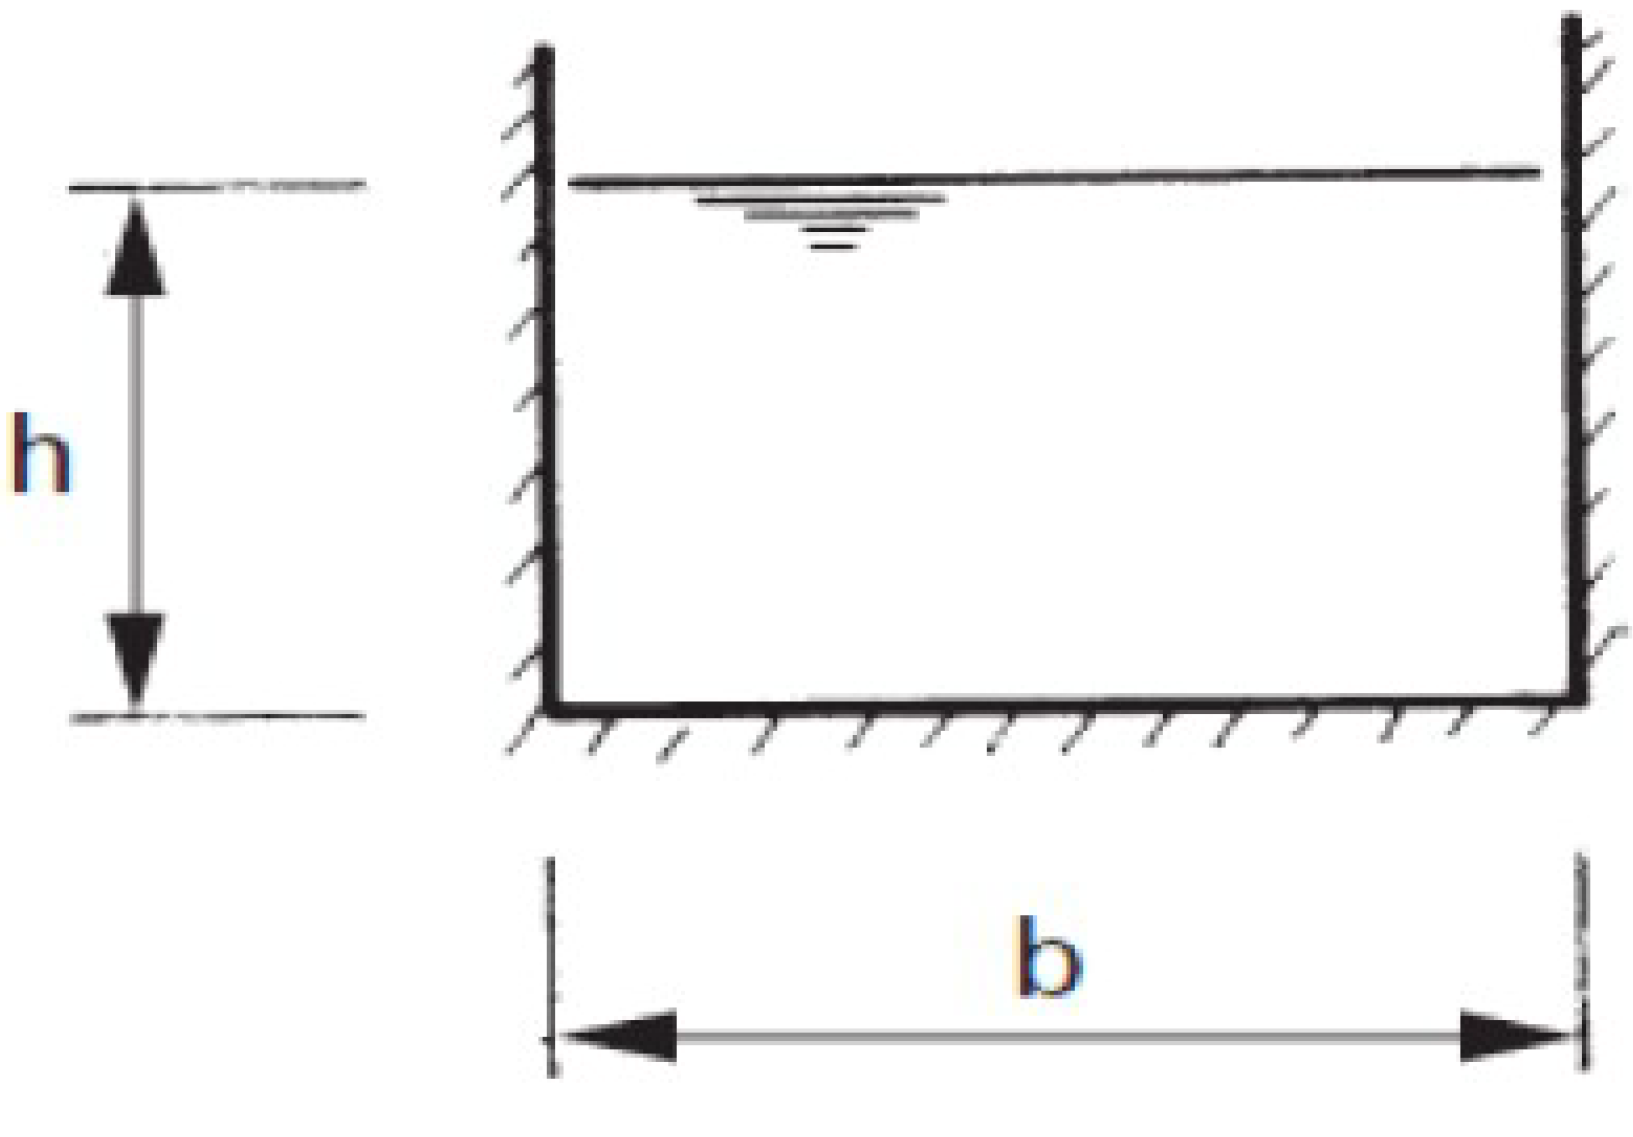
\includegraphics[width=0.9\textwidth, align=c]{images/Hydraulischer_Radius_Rechteck.png}
    \end{center}
\end{minipage}
\hfill
\vrule width 1pt % Vertikale Trennlinie mit 1pt Breite
\hfill
\begin{minipage}[c]{0.48\columnwidth}
    \myul{\textbf{Kreisqueerschnitt}}\\
    \begin{center}
        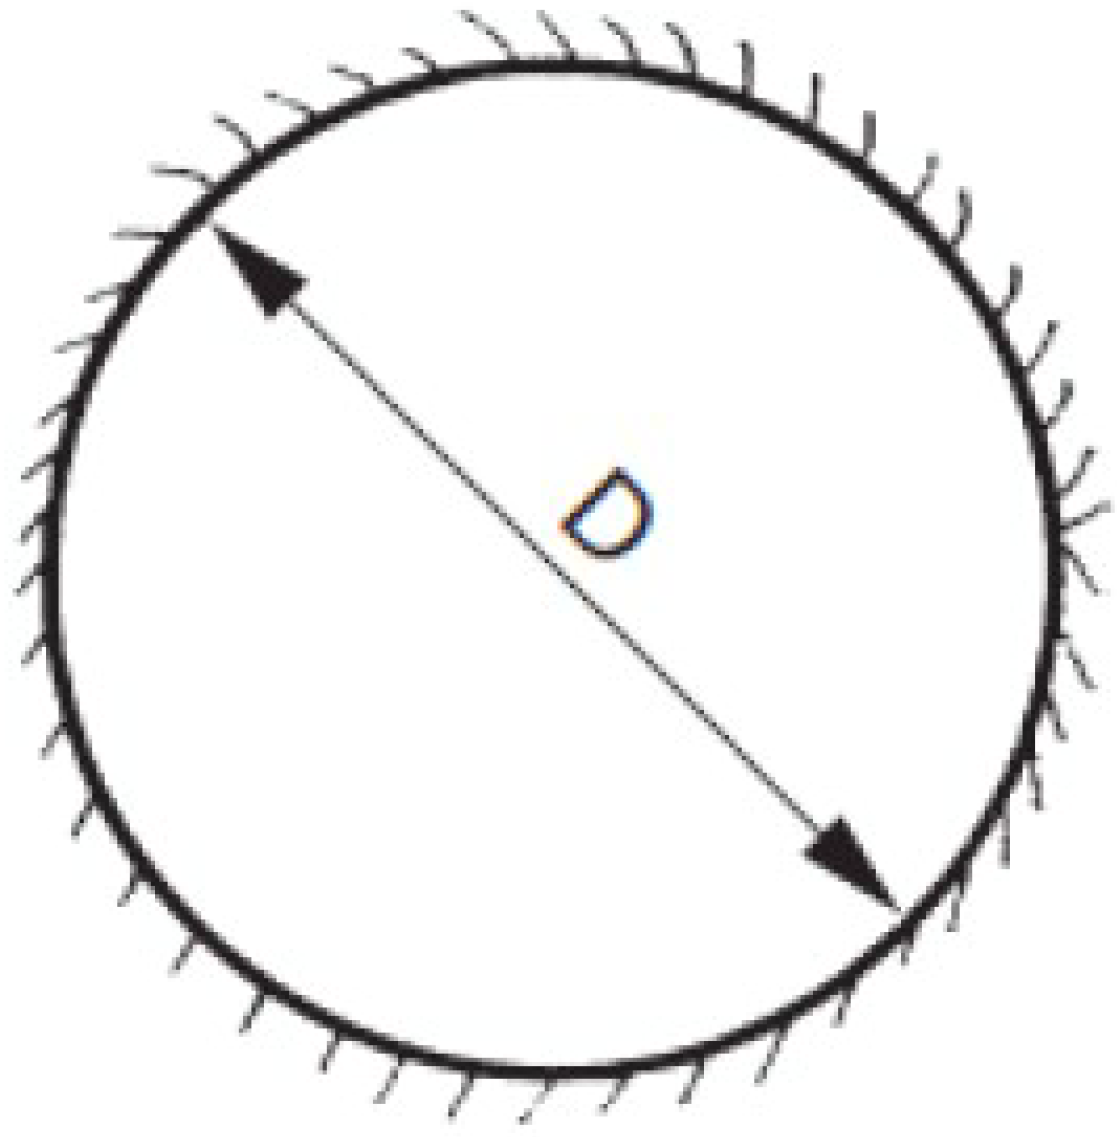
\includegraphics[width=0.65\textwidth, align=c]{images/Hydraulischer_Radius_Kreis.png}
    \end{center}
\end{minipage}

\vspace{0.25cm}

\begin{minipage}[c]{0.48\columnwidth}
    $\boxed{F = b \cdot h}$

    \vspace{0.15cm}

    $\boxed{P = b + 2 \cdot h}$

    \vspace{0.15cm}

    $\boxed{R_h = \frac{b \cdot h}{b + 2 \cdot h}}$ $\boxed{R_h = \frac{F}{P}}$
\end{minipage}
\hfill
\vrule width 1pt % Vertikale Trennlinie mit 1pt Breite
\hfill
\begin{minipage}[c]{0.48\columnwidth}
    $\boxed{F = \frac{D^2 \cdot \pi}{4}}$

    \vspace{0.15cm}

    $\boxed{P = D \cdot \pi}$

    \vspace{0.15cm}

    $\boxed{R_h = \frac{D}{4}}$ $\boxed{R_h = \frac{F}{P}}$
\end{minipage}

\vspace{0.15cm}

\renewcommand{\arraystretch}{1.2} % Erhöht Zeilenhöhe für bessere Lesbarkeit
\begin{tabular}{@{} l p {6cm} l @{}}
    $[F]$    & Abflussquerschnittsfläche         \dotfill & $\mathrm{m^2}$ \\
    $[P]$    & Benetzter Umfang                  \dotfill & $\mathrm{m}$ \\
    $[R_h]$  & Hydraulischer Radius              \dotfill & $\mathrm{m}$ \\
\end{tabular}





\subsection{Verlusthöhe durch Reibung}

$\boxed{h_{\text{v,r}} = \lambda \cdot \frac{L}{d_{\text{hy}}} \cdot \frac{v^2}{2 \cdot g} }
\quad
\boxed{h_{\text{v,r}} = \lambda \cdot \frac{L}{d_i} \cdot \frac{8 \cdot Q^2}{g \cdot \pi^2 \cdot d_i^4}}
\quad
\boxed{h_{\text{v,r}} = \frac{8 \cdot \lambda \cdot L \cdot Q^2}{g \cdot \pi^2 \cdot d_i^5}}$

\vspace{0.15cm}

\renewcommand{\arraystretch}{1.2} % Erhöht Zeilenhöhe für bessere Lesbarkeit
\begin{tabular}{@{} l p {6cm} l @{}}
    $[h_{\text{v,r}}]$  & Verlusthöhe durch Reibung      \dotfill & $\mathrm{m}$ \\
    $[L]$               & Länge                          \dotfill & $\mathrm{m}$ \\
    $[v_m]$             & Mittlere Geschwindigkeit       \dotfill & $\mathrm{\frac{m}{s}}$ \\
    $[Q]$               & Durchfluss                     \dotfill & $\mathrm{\frac{m^3}{s}}$ \\
    $[d_i]$             & Innendurchmesser               \dotfill & $\mathrm{m}$ \\
    $[d_{\text{hy}}]$   & Hydraulischer Durchmesser      \dotfill & $\mathrm{m}$ \\
    $[l_u]$             & Benetzter Umfang               \dotfill & $\mathrm{m}$ \\
    $[\lambda]$         & Verlustbeiwert                 \dotfill & $-$ \\
\end{tabular}


\vspace{0.15cm}

Zusammenhang des hydraulischen Durchmessers:

\vspace{0.15cm}

$
\boxed{d_{\text{hy}} = d_{\text{Kreisrohr}} = d_i = 4 \cdot R_{\text{hy}} = 4 \cdot \left(\frac{A}{l_u}\right)}
$



\subsection{Reynolds-Zahl $\text{Re}$}

Die Reynolds-Zahl $\text{Re}$ beschreibt das Verhältnis von Trägheitskräften zu Zähigkeitskräften in einer Strömung und wird wie folgt berechnet:

\vspace{0.15cm}

$\boxed{\text{Re} = \frac{v_m \cdot d_{\text{hy}}}{\nu}}$ \quad Bemerkung: $d_{\text{hy}} = d_{\text{Kreisrohr}} = d_i$

\vspace{0.15cm}

\renewcommand{\arraystretch}{1.2} % Erhöht Zeilenhöhe für bessere Lesbarkeit
\begin{tabular}{@{} l p {6cm} l @{}}
    $[\text{Re}]$     & Reynolds-Zahl (dimensionslos)                        \dotfill & $-$ \\
    $[v_m]$           & Mittlere Strömungsgeschwindigkeit                    \dotfill & $\mathrm{\frac{m}{s}}$ \\
    $[d_{\text{hy}}]$ & Hydraulischer Durchmesser                            \dotfill & $\mathrm{m}$ \\
    $[d_i]$           & Innendurchmesser (für Kreisrohr gleich $d_{\text{hy}}$) \dotfill & $\mathrm{m}$ \\
    $[\nu]$           & Kinematische Viskosität                              \dotfill & $\mathrm{\frac{m^2}{s}}$ \\
\end{tabular}



\newcolumn
\subsection{Verlustbeiwert }

$
\boxed{
\lambda = \left(\frac{1}{-2 \cdot \log \left( \frac{\varepsilon}{3{,}71} \right)}\right)^2
}
\quad
\boxed{
\lambda = \left(\frac{1}{-2 \cdot \log \left( \frac{k}{d_{hy} \cdot 3{,}71} \right)}\right)^2
}
$

\vspace{0.15cm}

\renewcommand{\arraystretch}{1.2}
\begin{tabular}{@{} l p{6cm} l @{}}
    $[\lambda]$ & Verlustbeiwert \dotfill & $-$ \\
    $[k]$ & äquivalente Rauheit \dotfill & mm \\
    $[d_{\text{hy}}]$ & Hydraulischer Durchmesser \dotfill & m \\
\end{tabular}



\subsection{Nettogefälle $H_n$}
$
\boxed{
H_n = H - \sum H_v - \frac{v^2}{2g}
}
\quad
\boxed{\sum H_v = C \cdot Q^2}
$

\vspace{0.15cm}

\renewcommand{\arraystretch}{1.2}
\begin{tabular}{@{} l p{6cm} l @{}}
    $[H_n]$       & Nettofallhöhe \dotfill & m \\
    $[H]$         & Bruttogefälle \dotfill & m \\
    $\left[\sum H_v\right]$ & Summe der hydraulischen Verluste \dotfill & m \\
    $[C]$         & Faktor bei Bestimmung der Verluste \dotfill & $\frac{\text{s}^{2}}{\text{m}^5}$ \\
    $[Q]$         & Volumenstrom \dotfill & $\frac{\text{m}^3}{\text{s}}$ \\
    $[v]$         & Strömungsgeschwindigkeit im Unterwasser \dotfill & $\frac{\text{m}}{\text{s}}$ \\
    $[g]$         & Erdbeschleunigung $g = 9{,}81$ \dotfill & $\frac{\text{m}}{\text{s}^2}$ \\
\end{tabular}



\subsection{Hydraulische Leistung $P_{\text{hyd}}$}

$
\boxed{P_{\text{hyd}} = \frac{m \cdot g \cdot H_n}{t} }
\quad
\boxed{P_{\text{hyd}} = \rho \cdot Q \cdot g \cdot H_n}
\quad
\boxed{\frac{\text{m}}{\text{t}} = \rho \cdot Q}
$

\vspace{0.15cm}

\renewcommand{\arraystretch}{1.2}
\begin{tabular}{@{} l p{6cm} l @{}}
    $[P_{\text{hyd}}]$  & Hydraulische Leistung \dotfill                & $\text{W}$ \\
    $[m]$               & Masse \dotfill                                & $\text{kg}$ \\
    $[g]$               & Erdbeschleunigung, $g = 9{,}81$ \dotfill      & $\frac{\text{m}}{\text{s}^2}$ \\
    $[H_n]$             & Nettofallhöhe \dotfill                        & $\text{m}$ \\
    $[t]$               & Zeit \dotfill                                & $\text{s}$ \\
    $[\rho]$            & Dichte des Wassers, $\rho = 1000$ \dotfill    & $\frac{\text{kg}}{\text{m}^3}$ \\
    $[Q]$               & Nutzwassermenge \dotfill                      & $\frac{\text{m}^3}{\text{s}}$\\ 
\end{tabular}



\subsection{Mechanische Leistung $P_{\text{mech}}$}

$
\boxed{P_{\text{mech}} = \eta_t \cdot P_{\text{hyd}}} 
\quad 
\boxed{P_{\text{mech}} = \eta_t \cdot \rho \cdot Q \cdot g \cdot H_n}
$

\vspace{0.15cm}

\renewcommand{\arraystretch}{1.2}
\begin{tabular}{@{} l p{7cm} l @{}}
    $[P_{\text{mech}}]$  & Mechanische Leistung an der Turbinen-Generator-Welle \dotfill & $\text{W}$ \\
    $[P_{\text{hyd}}]$   & Hydraulische Leistung \dotfill                               & $\text{W}$ \\
    $[\eta_t]$           & Turbinenwirkungsgrad \dotfill                               & $-$ \\
\end{tabular}



\subsection{Elektrische Leistung $P_{\text{el}}$}

$
\boxed{P_{\text{el}} = \eta_g \cdot P_{\text{mech}}} 
\quad 
\boxed{P_{\text{el}} = \eta_g \cdot \eta_t \cdot \rho \cdot Q \cdot g \cdot H_n}
$

\vspace{0.15cm}

\renewcommand{\arraystretch}{1.2}
\begin{tabular}{@{} l p{6cm} l @{}}
    $[P_{\text{el}}]$     & Elektrische Leistung an den Generatorklemmen \dotfill & $\text{W}$ \\
    $[P_{\text{mech}}]$   & Mechanische Leistung \dotfill                          & $\text{W}$ \\
    $[\eta_g]$            & Generatorwirkungsgrad \dotfill                         & $-$ \\
\end{tabular}



\subsection{Elektrische Energie $E$}

$
\boxed{E = \int P_{\text{el}} \cdot dt}
\quad
\boxed{E = \int \eta_g \cdot \eta_t \cdot Q \cdot H_n \cdot \rho \cdot g \cdot dt}
\quad
\boxed{E = \rho \cdot g \cdot \int \eta_g \cdot \eta_t \cdot Q \cdot H_n \cdot dt}
$

\vspace{0.15cm}

\renewcommand{\arraystretch}{1.2}
\begin{tabular}{@{} l p{6cm} l @{}}
    $[E]$               & Elektrische Energie \dotfill                           & $\text{Ws}$ \\
    $[P_{\text{el}}]$   & Elektrische Leistung \dotfill                          & $\text{W}$ \\
    $[\eta_g]$          & Generatorwirkungsgrad \dotfill                         & $-$ \\
    $[\eta_t]$          & Turbinenwirkungsgrad \dotfill                          & $-$ \\
    $[Q]$               & Nutzwassermenge \dotfill                               & $\frac{\text{m}^3}{\text{s}}$ \\
    $[H_n]$             & Nettofallhöhe \dotfill                                 & $\text{m}$ \\
    $[\rho]$            & Dichte des Wassers, $\rho = 1000$ \dotfill             & $\frac{\text{kg}}{\text{m}^3}$ \\
    $[g]$               & Erdbeschleunigung, $g = 9{,}81$ \dotfill               & $\frac{\text{m}}{\text{s}^2}$ \\
    $[t]$               & Zeit \dotfill                                           & $\text{s}$ \\
\end{tabular}
























































